% Options for packages loaded elsewhere
\PassOptionsToPackage{unicode}{hyperref}
\PassOptionsToPackage{hyphens}{url}
%
\documentclass{article}
\usepackage{amsmath,amssymb}
\usepackage{lmodern}
\usepackage{ifxetex,ifluatex}
\ifnum 0\ifxetex 1\fi\ifluatex 1\fi=0 % if pdftex
  \usepackage[T1]{fontenc}
  \usepackage[utf8]{inputenc}
  \usepackage{textcomp} % provide euro and other symbols
\else % if luatex or xetex
  \usepackage{unicode-math}
  \defaultfontfeatures{Scale=MatchLowercase}
  \defaultfontfeatures[\rmfamily]{Ligatures=TeX,Scale=1}
  \setmainfont[]{Open Sans}
\fi
% Use upquote if available, for straight quotes in verbatim environments
\IfFileExists{upquote.sty}{\usepackage{upquote}}{}
\IfFileExists{microtype.sty}{% use microtype if available
  \usepackage[]{microtype}
  \UseMicrotypeSet[protrusion]{basicmath} % disable protrusion for tt fonts
}{}
\makeatletter
\@ifundefined{KOMAClassName}{% if non-KOMA class
  \IfFileExists{parskip.sty}{%
    \usepackage{parskip}
  }{% else
    \setlength{\parindent}{0pt}
    \setlength{\parskip}{6pt plus 2pt minus 1pt}}
}{% if KOMA class
  \KOMAoptions{parskip=half}}
\makeatother
\usepackage{xcolor}
\IfFileExists{xurl.sty}{\usepackage{xurl}}{} % add URL line breaks if available
\IfFileExists{bookmark.sty}{\usepackage{bookmark}}{\usepackage{hyperref}}
\hypersetup{
  hidelinks,
  pdfcreator={LaTeX via pandoc}}
\urlstyle{same} % disable monospaced font for URLs
\usepackage[margin=1in]{geometry}
\usepackage{graphicx}
\makeatletter
\def\maxwidth{\ifdim\Gin@nat@width>\linewidth\linewidth\else\Gin@nat@width\fi}
\def\maxheight{\ifdim\Gin@nat@height>\textheight\textheight\else\Gin@nat@height\fi}
\makeatother
% Scale images if necessary, so that they will not overflow the page
% margins by default, and it is still possible to overwrite the defaults
% using explicit options in \includegraphics[width, height, ...]{}
\setkeys{Gin}{width=\maxwidth,height=\maxheight,keepaspectratio}
% Set default figure placement to htbp
\makeatletter
\def\fps@figure{htbp}
\makeatother
\setlength{\emergencystretch}{3em} % prevent overfull lines
\providecommand{\tightlist}{%
  \setlength{\itemsep}{0pt}\setlength{\parskip}{0pt}}
\setcounter{secnumdepth}{-\maxdimen} % remove section numbering
\usepackage{pdfpages}
\usepackage[default]{open sans}
\usepackage[T1]{fontenc}
\usepackage{graphicx} %ya estba este package x eso no compilaba cuando traté de poner
\usepackage{fancyhdr}
\usepackage{hyperref}
\usepackage{xcolor}
\usepackage{sidecap}
\usepackage[spanish]{babel}
\pagestyle{fancy}
\renewcommand{\headrulewidth}{0pt}
\fancyhead{}
\setlength{\headheight}{23pt}
\lhead{
\includegraphics[width=7cm,height=140cm]{"./logos/logo_oecc.pdf"}}
\fancyfoot{}
\lfoot{
\includegraphics[width=5.0cm,height=140cm]{"./logos/muni.jpg"}}
\rfoot{\thepage}
\definecolor{graycustom}{HTML}{7b7b7e}
\usepackage{floatrow}
\floatsetup[figure]{capposition=bottom} %ahí solucioné lo de la pos esto estaba en top 
\renewcommand{\arraystretch}{1.5}
\usepackage{svg}
\usepackage{amsmath}
\usepackage{booktabs}
\usepackage{longtable}
\usepackage{array}
\usepackage{multirow}
\usepackage{wrapfig}
\usepackage{float}
\usepackage{colortbl}
\usepackage{pdflscape}
\usepackage{tabu}
\usepackage{threeparttable}
\usepackage{threeparttablex}
\usepackage[normalem]{ulem}
\usepackage{makecell}
\usepackage{xcolor}
\ifluatex
\usepackage{selnolig}  % disable illegal ligatures
\fi
\setlength{\parindent}{14pt} %sangría

\author{}
\date{}

\usepackage[labelsep=endash]{caption} 

\AtBeginDocument{%
\renewcommand{\figurename}{Gráfico}
} %El comando \renewcommand{\figurename} no funciona solo porque se usa babel, usando \AtBeginDocument permite usar el comando 

\begin{document}


\textcolor{graycustom}{\Large Consideraciones metodológicas} \newline

El Observatorio Económico de la Municipalidad de Corrientes lleva a cabo
diversos informes sociodemográficos, utilizando como fuente principal la
base de microdatos de la Encuesta Permanente de Hogares elaborada por el
Instituto Nacional de Estadísticas y Censos (INDEC) y presentada con una
periodicidad trimestral. La misma se realiza a través de cuestionarios
presenciales que luego son volcados a bases de datos para ser utilizados
por el público en general.

A raíz del decreto N.º 297/2020 que establece el aislamiento social,
preventivo y obligatorio por la pandemia causada por el virus SARS-COV2,
y con el objetivo de no interrumpir el operativo continuo, el INDEC pasó
de la modalidad presencial a la telefónica para contactar y realizar la
entrevista a los hogares.

Esto implica que, a partir del segundo trimestre del 2020, el
relevamiento habitual de la EPH se ha visto afectado no solo por el
cambio de modalidad de entrevista, sino también por la cobertura de la
muestra, ya que la misma se redujo a las viviendas que tenían un número
de teléfono conocido o cuyo número se pudo obtener mediante estrategias
que no implicaban contacto personal. Ambos aspectos impactan en la
cantidad de hogares sin respuesta y ocasionan sesgos en las
estimaciones.

Gracias a los esfuerzos del INDEC para asegurar la difusión de las
estadísticas y aminorar los posibles sesgos producidos en los datos del
trimestre, el Observatorio Económico pudo llevar a cabo este informe.
Sin embargo, creemos oportuno realizar las aclaraciones metodológicas
antes descritas.

Por último, este trabajo se ha hecho considerando a los datos del primer
trimestre de 2021, con excepción de los apartados de informalidad por
sectores y calificación laboral por sectores, que se hicieron trabajando
en conjunto con las bases del cuarto trimestre del 2020.

\newpage

\textcolor{graycustom}{\Large Mercado de trabajo: 
Tasas e indicadores socioeconómicos (EPH)} \newline

Según las proyecciones de INDEC basadas en el último Censo de población,
la cantidad de habitantes total de la ciudad en el año 2021 es de 414927
personas. De ese total el 48.83\% son hombres y el restante 51.17\%,
mujeres.

De acuerdo con los datos publicados por el INDEC, basados también en el
último Censo Nacional de Población, Hogares y Viviendas (2010), la
población por edades se compone de la siguiente manera:

\begin{table}[htp!]

\caption{\label{tab:unnamed-chunk-6}Composición de la población}
\centering
\fontsize{9}{11}\selectfont
\begin{tabular}[t]{>{\raggedright\arraybackslash}p{18em}>{\raggedleft\arraybackslash}p{14em}>{\raggedleft\arraybackslash}p{14em}}
\toprule
\begingroup\fontsize{12}{14}\selectfont \cellcolor[HTML]{29aee4}{\textcolor{white}{\textbf{Edad}}}\endgroup & \begingroup\fontsize{12}{14}\selectfont \cellcolor[HTML]{29aee4}{\textcolor{white}{\textbf{Hombres}}}\endgroup & \begingroup\fontsize{12}{14}\selectfont \cellcolor[HTML]{29aee4}{\textcolor{white}{\textbf{Mujeres}}}\endgroup\\
\midrule
\cellcolor[HTML]{F0FFFF}{\cellcolor{gray!6}{0-14}} & \cellcolor[HTML]{F0FFFF}{\cellcolor{gray!6}{28.00\%}} & \cellcolor[HTML]{F0FFFF}{\cellcolor{gray!6}{25.00\%}}\\
15-24 & 21.00\% & 20.00\%\\
\cellcolor[HTML]{F0FFFF}{\cellcolor{gray!6}{25-34}} & \cellcolor[HTML]{F0FFFF}{\cellcolor{gray!6}{16.00\%}} & \cellcolor[HTML]{F0FFFF}{\cellcolor{gray!6}{16.00\%}}\\
35-44 & 11.00\% & 12.00\%\\
\cellcolor[HTML]{F0FFFF}{\cellcolor{gray!6}{45-59}} & \cellcolor[HTML]{F0FFFF}{\cellcolor{gray!6}{15.00\%}} & \cellcolor[HTML]{F0FFFF}{\cellcolor{gray!6}{15.00\%}}\\
\addlinespace
Mayor o igual a 60 & 9.00\% & 12.00\%\\
\bottomrule
\end{tabular}
\end{table}


\begin{figure}
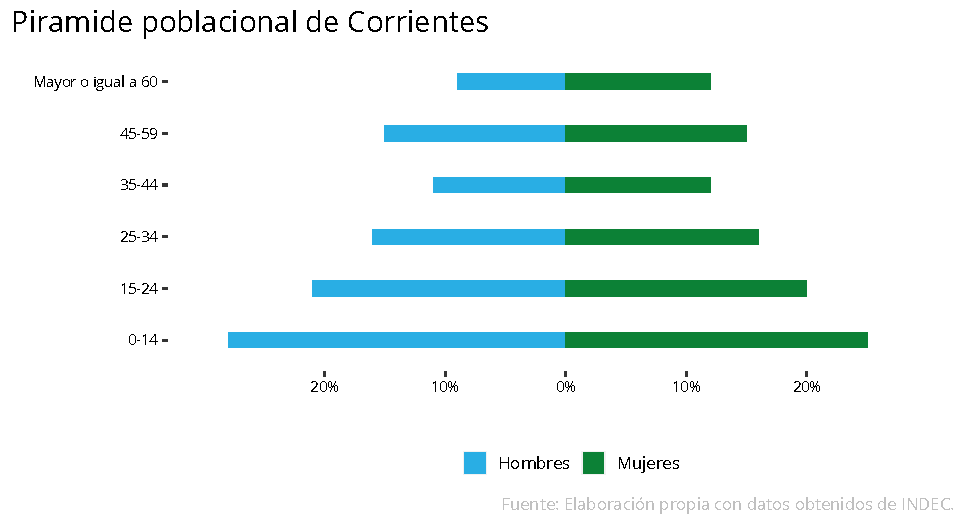
\includegraphics{Informe-Mercado-Laboral_files/figure-latex/unnamed-chunk-7-1.pdf}
\caption{} %el asterisco es para q no diga figura 1
\end{figure}

\newpage


\textcolor{graycustom}{\Large Indicadores de participación laboral} \newline

Los resultados para primer trimestre de 2021 para la Ciudad de
Corrientes muestran que la tasa de actividad es del 43.99\%.

Del total de la PEA, el 53.81\% son hombres y el 46.19\% mujeres. Por
otro lado, se observa que del total de mujeres el 38.99\% forman parte
de la PEA, mientras que en el caso de los hombres el porcentaje que
forma parte de la PEA alcanza el 49.44\%.

La población económicamente activa (PEA), a su vez, está compuesta por
los ocupados y desocupados. Este último grupo presiona activamente sobre
el mercado laboral en búsqueda de una ocupación.

La definición vista de PEA, no incluye al trabajo no remunerado
(doméstico, voluntario y de subsistencia). Esto implica que, en la
medición de la actividad de la EPH, no se considera activa a la
población que realiza producción o tratamiento de bienes exclusivamente
para autoconsumo. Esto trae inconvenientes en cuanto a la subestimación
de la participación femenina en la actividad económica. Por la
importancia que tiene este tópico en las brechas de género, el tema es
tratado especialmente en el ``Informe de Género'' realizado por el
Observatorio Económico de la Ciudad de Corrientes.

A continuación, se aprecian los porcentajes, tanto de hombres como de
mujeres, que forman parte de la PEA, desagregados por rangos de edad.


\begin{table}[hbp!]

\caption{\label{tab:unnamed-chunk-5}Participación laboral por sexo y edad}
\centering
\fontsize{9}{11}\selectfont
\begin{tabular}[t]{>{\raggedright\arraybackslash}p{18em}>{\raggedleft\arraybackslash}p{14em}>{\raggedleft\arraybackslash}p{14em}}
\toprule
\begingroup\fontsize{12}{14}\selectfont \cellcolor[HTML]{29aee4}{\textcolor{white}{\textbf{Edad}}}\endgroup & \begingroup\fontsize{12}{14}\selectfont \cellcolor[HTML]{29aee4}{\textcolor{white}{\textbf{Hombres}}}\endgroup & \begingroup\fontsize{12}{14}\selectfont \cellcolor[HTML]{29aee4}{\textcolor{white}{\textbf{Mujeres}}}\endgroup\\
\midrule
\cellcolor[HTML]{F0FFFF}{\cellcolor{gray!6}{15-24 años}} & \cellcolor[HTML]{F0FFFF}{\cellcolor{gray!6}{29.18\%}} & \cellcolor[HTML]{F0FFFF}{\cellcolor{gray!6}{33.35\%}}\\
25-34 años & 86.27\% & 62.57\%\\
\cellcolor[HTML]{F0FFFF}{\cellcolor{gray!6}{35-44 años}} & \cellcolor[HTML]{F0FFFF}{\cellcolor{gray!6}{93.29\%}} & \cellcolor[HTML]{F0FFFF}{\cellcolor{gray!6}{73.99\%}}\\
45-59 años & 92.66\% & 70.07\%\\
\cellcolor[HTML]{F0FFFF}{\cellcolor{gray!6}{Igual o mayor a 60 años}} & \cellcolor[HTML]{F0FFFF}{\cellcolor{gray!6}{34.58\%}} & \cellcolor[HTML]{F0FFFF}{\cellcolor{gray!6}{11.32\%}}\\
\bottomrule
\end{tabular}
\end{table}

\newpage
\begin{figure}
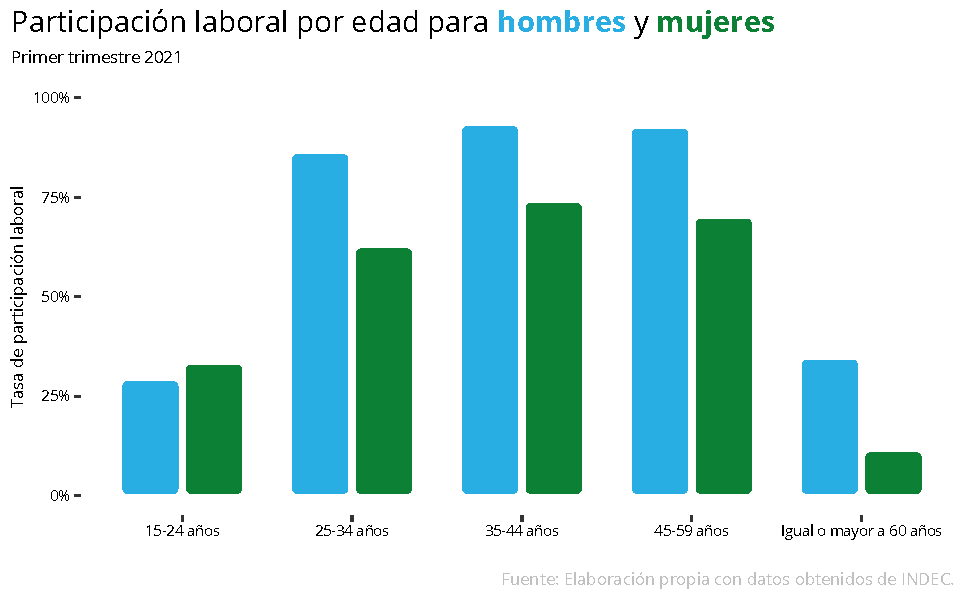
\includegraphics{Informe-Mercado-Laboral_files/figure-latex/unnamed-chunk-13-1.pdf}
\caption{} 
\end{figure}


Se puede observar que, con excepción al rango etario de 15 a 24 años,
existe una brecha en la tasa de actividad que muestra que hay menos
mujeres participando en el mercado laboral, en comparación a los
hombres.

A modo de observación, para ambos sexos, el porcentaje máximo de
participación se encuentra entre los 35 a 44 años.

Tanto en la tabla como en el Gráfico 3 se exponen los porcentajes tanto
de hombres como de mujeres pertenecientes a la PEA, desagregados por el
nivel de educación alcanzado, junto con las respectivas brechas. Se
entiende como brecha a la diferencia entre el porcentaje de hombres y
mujeres que conforman la PEA para cada nivel educativo.

\begin{table}[htbp!]

\caption{\label{tab:unnamed-chunk-15}Participación laboral por sexo y nivel educativo}
\centering
\fontsize{9}{11}\selectfont
\begin{tabular}[t]{>{\raggedright\arraybackslash}p{12em}>{\raggedleft\arraybackslash}p{10em}>{\raggedleft\arraybackslash}p{10em}>{\raggedleft\arraybackslash}p{10em}}
\toprule
\begingroup\fontsize{12}{14}\selectfont \cellcolor[HTML]{29aee4}{\textcolor{white}{\textbf{Nivel}}}\endgroup & \begingroup\fontsize{12}{14}\selectfont \cellcolor[HTML]{29aee4}{\textcolor{white}{\textbf{Hombres}}}\endgroup & \begingroup\fontsize{12}{14}\selectfont \cellcolor[HTML]{29aee4}{\textcolor{white}{\textbf{Mujeres}}}\endgroup & \begingroup\fontsize{12}{14}\selectfont \cellcolor[HTML]{29aee4}{\textcolor{white}{\textbf{Brecha}}}\endgroup\\
\midrule
\cellcolor[HTML]{F0FFFF}{\cellcolor{gray!6}{Primaria Completa}} & \cellcolor[HTML]{F0FFFF}{\cellcolor{gray!6}{48.48\%}} & \cellcolor[HTML]{F0FFFF}{\cellcolor{gray!6}{21.25\%}} & \cellcolor[HTML]{F0FFFF}{\cellcolor{gray!6}{27.23\%}}\\
Secundaria Completa & 65.82\% & 56.18\% & 9.64\%\\
\cellcolor[HTML]{F0FFFF}{\cellcolor{gray!6}{Superior Completo}} & \cellcolor[HTML]{F0FFFF}{\cellcolor{gray!6}{83.88\%}} & \cellcolor[HTML]{F0FFFF}{\cellcolor{gray!6}{73.90\%}} & \cellcolor[HTML]{F0FFFF}{\cellcolor{gray!6}{9.98\%}}\\
\bottomrule
\end{tabular}
\end{table}


\newpage
\begin{figure}
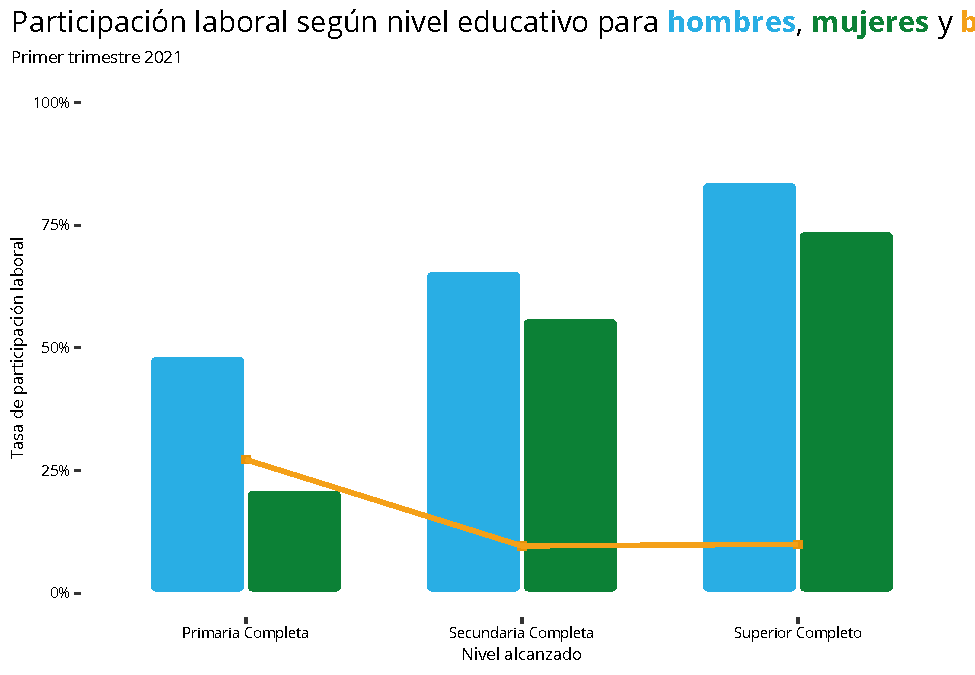
\includegraphics{Informe-Mercado-Laboral_files/figure-latex/unnamed-chunk-16-1.pdf}
\caption{}
\end{figure}

La mayor brecha de participación entre sexos se encuentra en el nivel
primario.

Los valores que se presentan y grafican a continuación corresponden al
promedio de horas semanales que trabajan tanto hombres como mujeres,
desagregados por edad.

\begin{table}[hp!]

\caption{\label{tab:unnamed-chunk-19}Carga laboral semanal por sexo y edad}
\centering
\fontsize{9}{11}\selectfont
\begin{tabular}[t]{>{\raggedright\arraybackslash}p{12em}>{\raggedleft\arraybackslash}p{10em}>{\raggedleft\arraybackslash}p{10em}>{\raggedleft\arraybackslash}p{10em}}
\toprule
\begingroup\fontsize{12}{14}\selectfont \cellcolor[HTML]{29aee4}{\textcolor{white}{\textbf{Edad}}}\endgroup & \begingroup\fontsize{12}{14}\selectfont \cellcolor[HTML]{29aee4}{\textcolor{white}{\textbf{Hombres}}}\endgroup & \begingroup\fontsize{12}{14}\selectfont \cellcolor[HTML]{29aee4}{\textcolor{white}{\textbf{Mujeres}}}\endgroup & \begingroup\fontsize{12}{14}\selectfont \cellcolor[HTML]{29aee4}{\textcolor{white}{\textbf{Brecha}}}\endgroup\\
\midrule
\cellcolor[HTML]{F0FFFF}{\cellcolor{gray!6}{15-24 años}} & \cellcolor[HTML]{F0FFFF}{\cellcolor{gray!6}{39.34}} & \cellcolor[HTML]{F0FFFF}{\cellcolor{gray!6}{26.02}} & \cellcolor[HTML]{F0FFFF}{\cellcolor{gray!6}{13.33}}\\
25-34 años & 38.80 & 30.44 & 8.35\\
\cellcolor[HTML]{F0FFFF}{\cellcolor{gray!6}{35-44 años}} & \cellcolor[HTML]{F0FFFF}{\cellcolor{gray!6}{38.97}} & \cellcolor[HTML]{F0FFFF}{\cellcolor{gray!6}{30.77}} & \cellcolor[HTML]{F0FFFF}{\cellcolor{gray!6}{8.20}}\\
45-59 años & 39.20 & 27.21 & 11.99\\
\cellcolor[HTML]{F0FFFF}{\cellcolor{gray!6}{Igual o mayor a 60 años}} & \cellcolor[HTML]{F0FFFF}{\cellcolor{gray!6}{33.71}} & \cellcolor[HTML]{F0FFFF}{\cellcolor{gray!6}{21.19}} & \cellcolor[HTML]{F0FFFF}{\cellcolor{gray!6}{12.52}}\\
\bottomrule
\end{tabular}
\end{table}


\begin{figure}
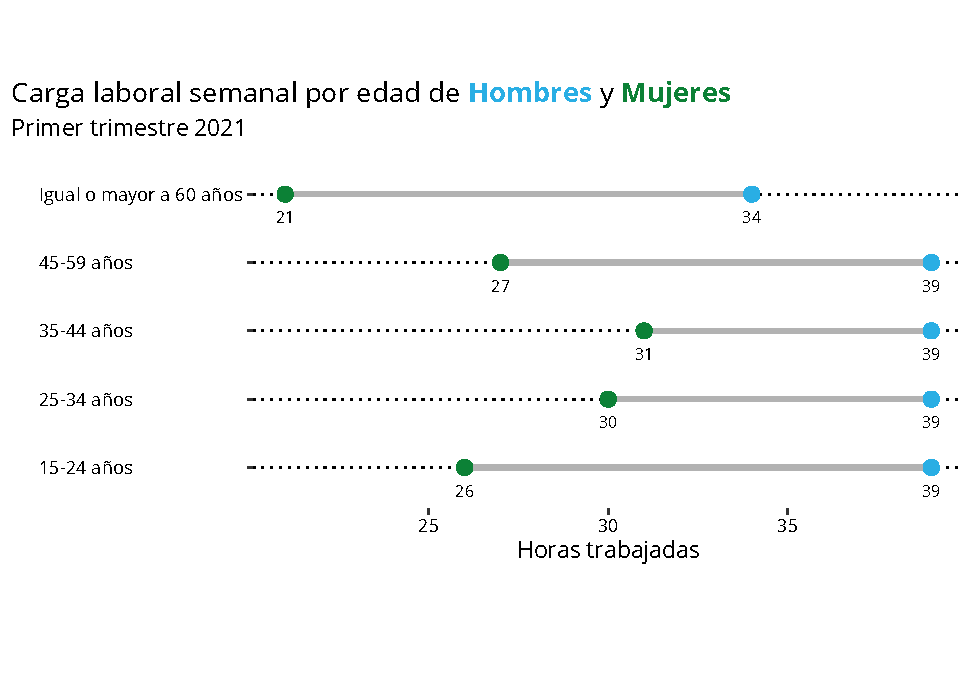
\includegraphics{Informe-Mercado-Laboral_files/figure-latex/unnamed-chunk-20-1.pdf}
\caption{} 
\end{figure}

\newpage
Se observa que para todos los rangos etarios los hombres tienen una
carga laboral superior a las mujeres, dándose las brechas más grandes
para el primer caso, de 13.33 horas en promedio y para los mayores a 60
años de 12.52 horas.

\newpage

\textcolor{graycustom}{\Large Tasas de empleo y desocupación} \newline
\begin{figure}
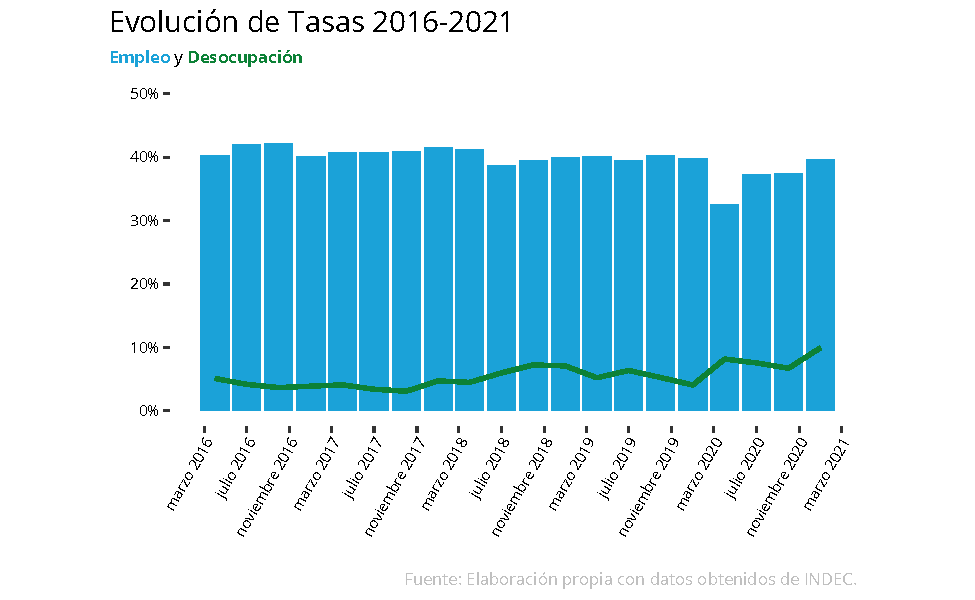
\includegraphics{Informe-Mercado-Laboral_files/figure-latex/unnamed-chunk-23-1.pdf}
\caption{} 
\end{figure}


La tasa de empleo en la Ciudad de Corrientes para el
trimestre en cuestión asciende 39.63\%, esta tasa se calcula como el
cociente entre el total de ocupados y la población total de referencia.
Por su parte, la tasa de desocupación, que se calcula como el cociente
entre desocupados y la Población Económicamente Activa (PEA), es del
9.93\%.

\newpage

\textcolor{graycustom}{\Large Empleo público y privado} \newline

Del total de empleados de la ciudad, el porcentaje de empleados públicos
es de 24.95\% siendo 74.19\% trabajadores pertenecientes al sector
privado, quedando el ínfimo porcentaje restante sin especificar.


\begin{figure}[hbp!]
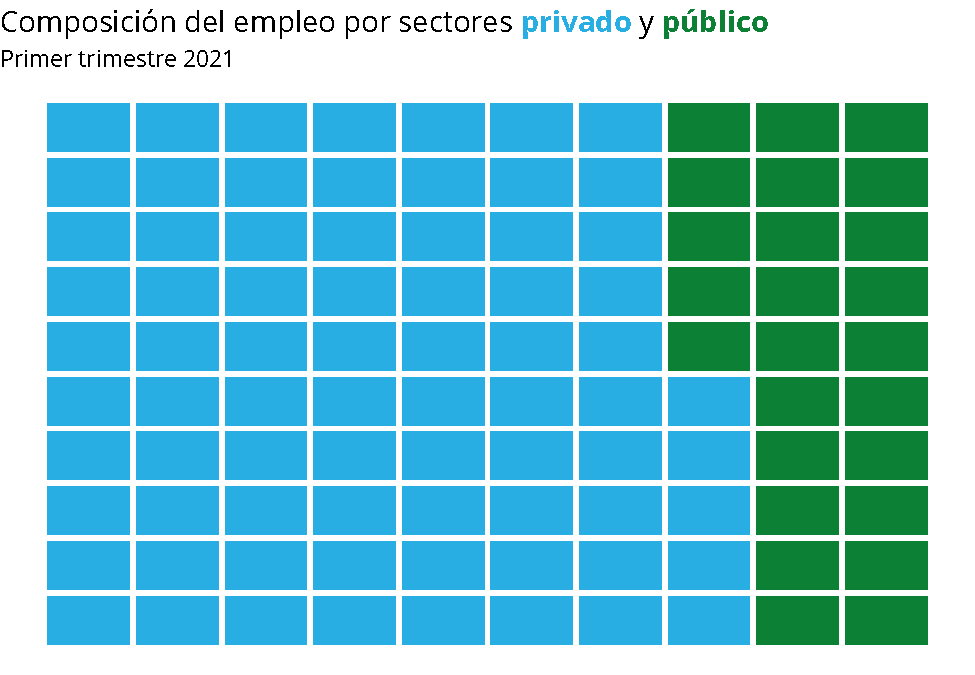
\includegraphics{Informe-Mercado-Laboral_files/figure-latex/unnamed-chunk-25-1.pdf}
\caption{}
\end{figure}


En el sector público, el promedio de edad de los trabajadores es de 45
años, mientras que en el sector privado es de 38, trabajando 28 y 36
horas semanales en promedio en el sector público y privado,
respectivamente. A su vez, el Estado cuenta con una calificación laboral
del 53.67\%, mientras que el sector privado, tan solo del 23.81\%.

Por otro lado, el sector público se compone de una participación de
50.62\% hombres y 49.38\% mujeres. Mientras que, en el sector privado,
el porcentaje de hombres llega al 55.12\%.


\newpage
\begin{figure}
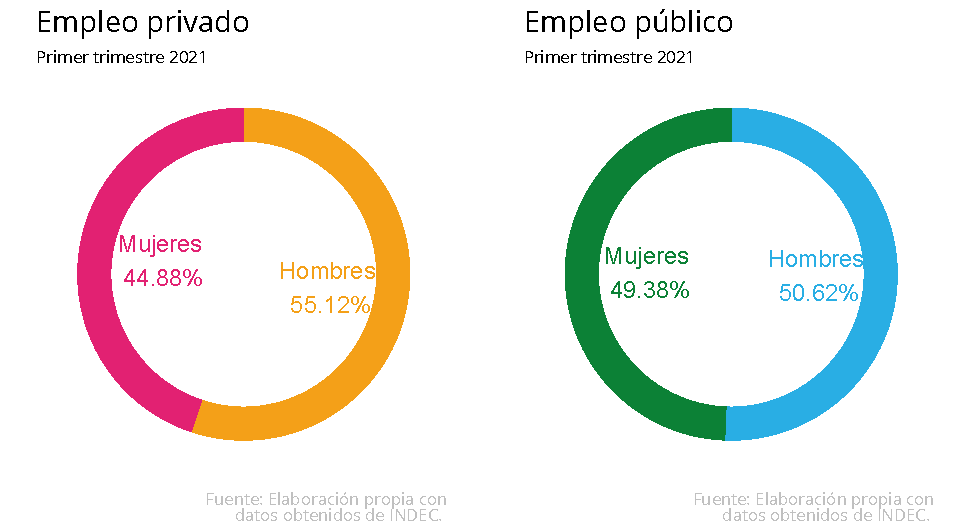
\includegraphics{Informe-Mercado-Laboral_files/figure-latex/unnamed-chunk-31-1.pdf}\caption{} 
\end{figure}

En términos de la composición por sectores en el empleo público (Gráfico
9), la ``Administración Pública'' cuenta con la mayor participación
laboral, ocupando un 44.54\% del total de empleos públicos, seguida por
la ``Enseñanza'' en todos sus niveles, con un 30.70\% del total de
empleos y en tercer lugar el rubro de la ``Salud'', con un 15.07\% de la
participación.

\begin{figure}
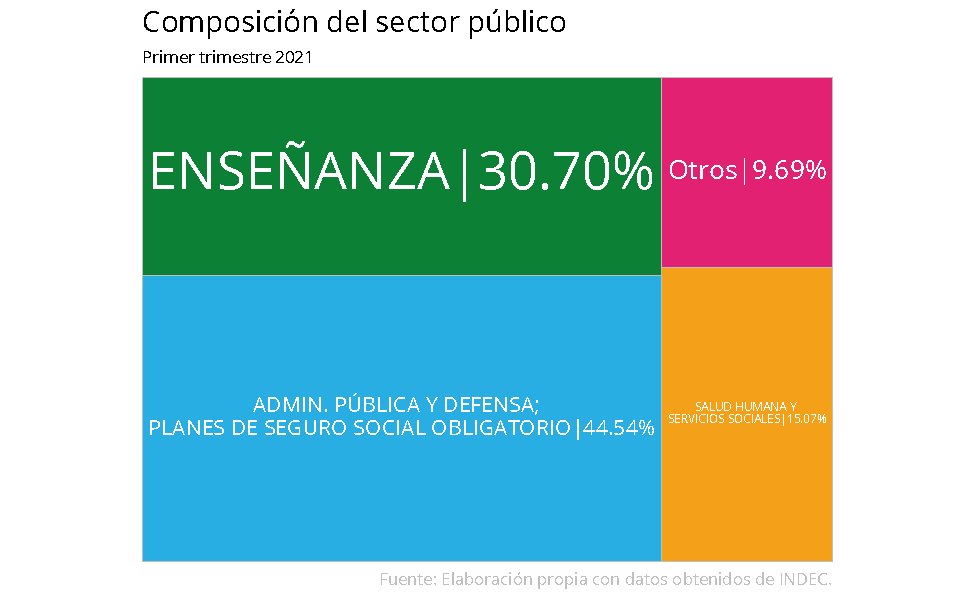
\includegraphics{Informe-Mercado-Laboral_files/figure-latex/unnamed-chunk-33-1.pdf}
\caption{} 
\end{figure}

\newpage

\textcolor{graycustom}{\Large Tasas de informalidad laboral} \newline

Para el análisis del trabajo no registrado, se construye una tasa de
informalidad que relaciona la cantidad de personas que poseen un empleo
en relación de dependencia, pero no perciben aportes jubilatorios por el
mismo. 

En la tabla y el gráfico siguiente se presenta información
relacionada a la población que trabaja de manera informal desagregada
tanto por edad como por sexo:

\begin{table}[hbp!]

\caption{\label{tab:unnamed-chunk-37}Informalidad laboral por sexo y edad}
\centering
\fontsize{9}{11}\selectfont
\begin{tabular}[t]{>{\raggedright\arraybackslash}p{18em}>{\raggedleft\arraybackslash}p{14em}>{\raggedleft\arraybackslash}p{14em}}

\begingroup\fontsize{12}{14}\selectfont \cellcolor[HTML]{29aee4}{\textcolor{white}{\textbf{Edad}}}\endgroup & \begingroup\fontsize{12}{14}\selectfont \cellcolor[HTML]{29aee4}{\textcolor{white}{\textbf{Hombres}}}\endgroup & \begingroup\fontsize{12}{14}\selectfont \cellcolor[HTML]{29aee4}{\textcolor{white}{\textbf{Mujeres}}}\endgroup\\
\midrule
\cellcolor[HTML]{F0FFFF}{\cellcolor{gray!6}{15-24 años}} & \cellcolor[HTML]{F0FFFF}{\cellcolor{gray!6}{100.00\%}} & \cellcolor[HTML]{F0FFFF}{\cellcolor{gray!6}{77.85\%}}\\
25-34 años & 49.67\% & 57.43\%\\
\cellcolor[HTML]{F0FFFF}{\cellcolor{gray!6}{35-44 años}} & \cellcolor[HTML]{F0FFFF}{\cellcolor{gray!6}{25.25\%}} & \cellcolor[HTML]{F0FFFF}{\cellcolor{gray!6}{31.85\%}}\\
45-59 años & 27.16\% & 29.54\%\\
\cellcolor[HTML]{F0FFFF}{\cellcolor{gray!6}{+60 años}} & \cellcolor[HTML]{F0FFFF}{\cellcolor{gray!6}{37.04\%}} & \cellcolor[HTML]{F0FFFF}{\cellcolor{gray!6}{37.90\%}}\\

\end{tabular}
\end{table}

\begin{figure}
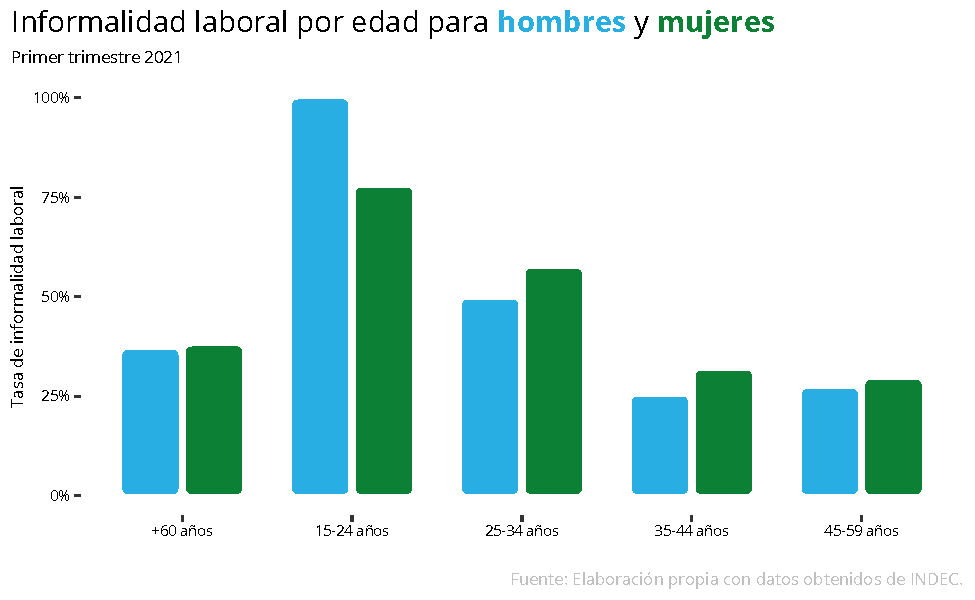
\includegraphics{Informe-Mercado-Laboral_files/figure-latex/unnamed-chunk-38-1.pdf}
\caption{} 
\end{figure}

\newpage
Al analizar la informalidad laboral por sector de actividad, los menores
valores se encuentran en el sector de enseñanza (4.68\%); el sector de
administración pública y defensa, planes de seguro social obligatorio
(8.81\%); actividades financieras y de seguro(10.48\%) el sector de
información y comunicación (14.86\%); suministro de Agua,
alcantarillado, gestión de desechos y actividades de saneamiento
(19.12\%) y Actividades de Organizaciones y Organismos
Extraterritoriales (23.79\%). Por otro lado, los valores más altos están
en el sector de servicio doméstico y actividades para consumo propio
(82.49\%); actividades científicas y técnicas (80.61\%); actividades
inmobiliarias (72.51\%); el de construcción (71.02\%) e industria
manufacturera (63.87\%).


\begin{figure}
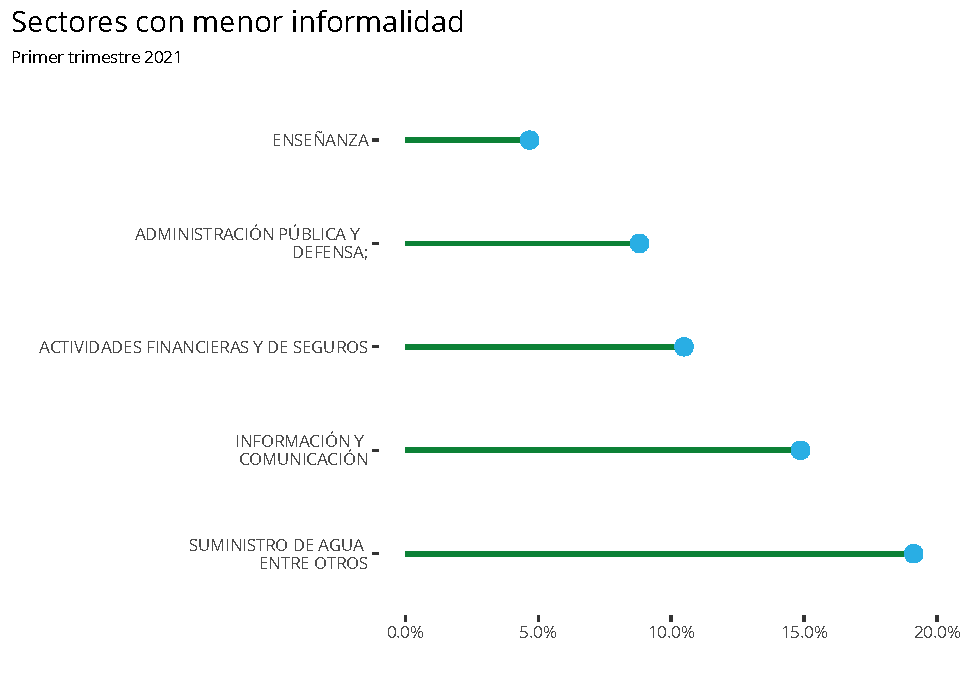
\includegraphics{Informe-Mercado-Laboral_files/figure-latex/unnamed-chunk-40-1.pdf}
\caption{} 
\end{figure}
\begin{figure}
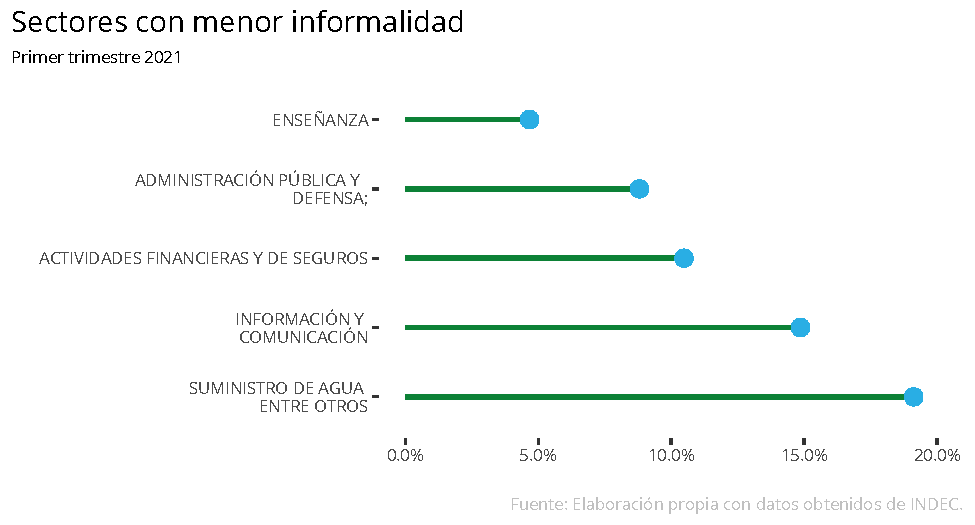
\includegraphics{Informe-Mercado-Laboral_files/figure-latex/unnamed-chunk-41-1.pdf}
\caption{} 
\end{figure}


\newpage
\textcolor{graycustom}{\Large Tasas de calificación laboral} \newline

En la EPH se clasifica a los empleados en cuatro categorías:
profesionales, técnicos, operarios y trabajadores no calificados. A
efectos de este análisis se consideran calificados a los profesionales o
técnicos, mientras que a los no calificados se le suman los operarios
para determinar la categoría final de no calificados.

Del total de la población de la ciudad, solo el 31.43\% son calificados,
mientras que el 68.57\% restante son no calificados. Del total de los
hombres, el 29.92\% son calificados, mientras que del total de las
mujeres el porcentaje de calificación es del 33\%.

Al analizar la calificación laboral por sector de actividad los valores
más altos están en los rubros de profesionales, científicos y técnicos
(88.54\%); enseñanza (85.08\%); información y comunicación (80.77\%);
arte, entretenimiento y recreación (69.31\%); y salud humana y servicios
sociales (60.41\%).
\begin{figure}
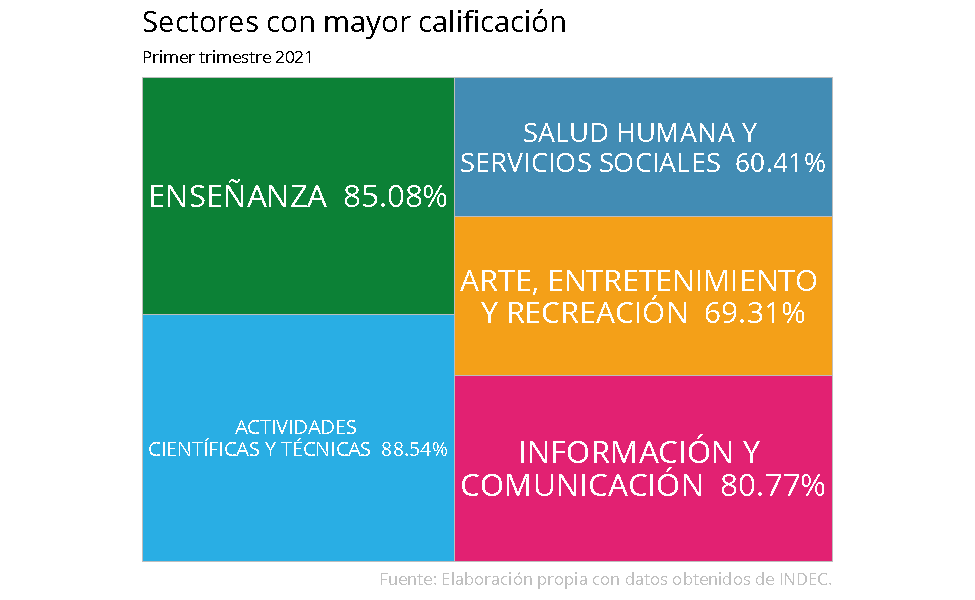
\includegraphics{Informe-Mercado-Laboral_files/figure-latex/unnamed-chunk-45-1.pdf}
\caption{} 
\end{figure}
\end{document}
